\renewcommand{\VERAPaperPDFTitle}{VERA: Support-Aware Certification of Representation Edits Under Deployment Shift}
\renewcommand{\VERAPaperDisplayTitle}{VERA: Support-Aware Certification of Representation Edits\\Under Deployment Shift}
\renewcommand{\VERAPaperPDFSubject}{Support-aware certification of representation edits under deployment shift}
\providecommand{\ControlledShiftAbstractResult}{The first preregistered controlled-shift primary made 38 VERA deployments with 0 violations but failed its usefulness gate because the 95\% lower bound was 15.1\%. We then locked an independent, non-pooling follow-up before seeds 109--172. At the higher preregistered 8,000-observation budget, validation selection violated 24/186 deployed decisions while VERA deployed 59 edits with 0 shifted-contract violations, retained 59/183 oracle-safe opportunities (32.2\%, 95\% CI [27.5\%, 36.8\%]), and passed every registered follow-up gate.}
\providecommand{\ControlledPrimaryResult}{The first controlled-shift primary remains a disclosed mixed result: validation selection violated 19/186 deployed decisions, whereas the VERA vector envelope deployed 38 edits with 0 violations; safety, paired reduction, and vector/common advantage passed, but usefulness failed because safe retention was 38/187 (20.3\%) with 95\% seed-bootstrap CI [15.1\%, 25.5\%]. The independent post-failure follow-up is not pooled with that result, but it passed as a new locked test: validation selection violated 24/186 deployed decisions, VERA deployed 59 edits with 0 violations, and the paired sign test had 22 favorable seed clusters, 0 adverse, and $p=4.77e-07$.}
\providecommand{\ControlledSafetyResult}{In the independent follow-up, the rotating-sentinel safety gate passed with 0/64 false acceptances and a one-sided 95\% Clopper--Pearson upper bound of 4.6\%. Across all follow-up VERA vector deployments, shifted-law violations were 0/59.}
\providecommand{\ControlledRetentionResult}{Follow-up safe retention was 59/183 (32.2\%) with 95\% seed-bootstrap CI [27.5\%, 36.8\%], clearing the registered 20\% lower-bound gate. The common-radius rule retained 11/183 (6.0\%); the vector/common ratio was 5.36 with 95\% interval [3.5, 10.4], so the vector-advantage gate also passed.}
\providecommand{\ControlledAllocationResult}{The follow-up evidence-size sweep shows the effect of certification budget: at $\Gamma=1.1$, the targeted vector rule retained 2/183, 22/183, 51/183, and 59/183 oracle-safe opportunities at budgets 1,000, 2,000, 4,000, and 8,000, respectively, with zero deployed violations in every row. The 8,000-observation row was locked as the independent follow-up primary before seeds 109--172 were run.}
\providecommand{\ControlledEvidenceResult}{The follow-up geometry remains narrow but useful: among 59 vector deployments, the median common radius was 1.040, with range [1.002, 1.183]. The most frequent limiting coordinate was target::environment=0 (39 of 59 deployments), followed by source::0 (14 of 59).}
\providecommand{\ControlledGaitResult}{The follow-up did not deploy uniformly across domains: VERA vector abstained on Bios and CivilComments, deployed 14/64 GaitPDB seed decisions and 45/64 Waterbirds seed decisions, and had zero shifted-contract violations on every deployment. This is the intended abstain-or-edit behavior under the supported-envelope contract.}
\providecommand{\ControlledHeldoutResult}{The held-out boosted-tree stress remains outside the formal registered attacker guarantee: it found 5 violations among 59 follow-up vector deployments (8.5\% unsafe), so the paper reports it as portfolio-scope stress rather than as a coverage claim.}
\providecommand{\ControlledNegativeResults}{The first 64-seed primary's failed usefulness gate remains mandatory negative evidence and is not rescued, pooled, or replaced by the follow-up. The independent follow-up is reported as a separately locked post-failure confirmation at the preregistered higher evidence budget; secondary threshold-stress, held-out-attacker, and dataset-specific rows remain ineligible as primary substitutes.}
\providecommand{\ControlledMainResultTable}{\begin{table*}[t]
\centering
\small
\begin{tabular}{@{}lrrrr@{}}
\toprule
Rule & Deployments & Viol./deployed & Safe retention & Median radius \\
\midrule
Always deploy & 256/256 (100.0\%) & 128/256 (50.0\%) & 128/183 (69.9\%) & NA \\
Validation selection & 186/256 (72.7\%) & 24/186 (12.9\%) & 162/183 (88.5\%) & NA \\
IID LTT & 109/256 (42.6\%) & 0/109 (0.0\%) & 109/183 (59.6\%) & NA \\
Robust point estimate & 98/256 (38.3\%) & 3/98 (3.1\%) & 95/183 (51.9\%) & NA \\
Scalar robust certificate & 256/256 (100.0\%) & 126/256 (49.2\%) & 130/183 (71.0\%) & NA \\
VERA fixed profile & 67/256 (26.2\%) & 0/67 (0.0\%) & 67/183 (36.6\%) & NA \\
VERA vector envelope & 59/256 (23.0\%) & 0/59 (0.0\%) & 59/183 (32.2\%) & 1.04 \\
VERA common radius & 11/256 (4.3\%) & 0/11 (0.0\%) & 11/183 (6.0\%) & NA \\
External oracle & 183/256 (71.5\%) & 0/183 (0.0\%) & 183/183 (100.0\%) & NA \\
\bottomrule
\end{tabular}
\caption{Independent post-failure controlled-shift follow-up at $\Gamma=1.1$, budget 8,000, and targeted allocation with a 15\% evidence floor. Safe retention is retained oracle-safe opportunities over all oracle-safe opportunities. Unlike the first 64-seed primary, this independently locked follow-up passes every registered gate.}
\label{tab:controlled-followup}
\end{table*}
}
\providecommand{\ControlledMainResultFigure}{\begin{figure}[t]\centering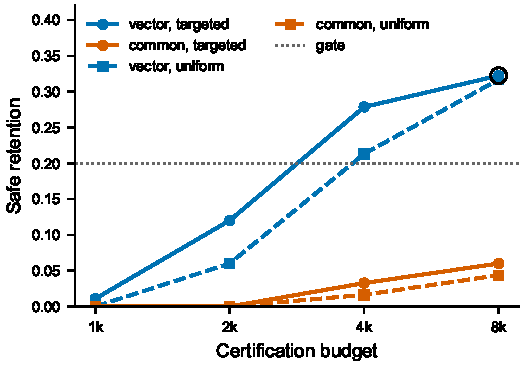
\includegraphics[width=\columnwidth]{../../figures/vera_controlled_shift_followup_budget_curve.pdf}\caption{Independent follow-up evidence-size sensitivity at $\Gamma=1.1$. The circled point is the locked follow-up primary vector rule (budget 8,000, targeted allocation), which clears the registered usefulness gate with zero shifted-contract violations. Lower budgets and uniform allocation are reported as sensitivity analyses.}\label{fig:controlled-followup-budget}\end{figure}}
